\documentclass[11pt, a4paper]{article} % setsfont size and layout

%% required packages %%

\usepackage[margin=2.5cm]{geometry} % margins
\usepackage[english]{babel} % language (replace with german or ngerman for german texts)
\usepackage[utf8]{inputenc} % Umlaute
\usepackage{amsmath}		% math formulas
\usepackage{graphicx}		% graphics
\usepackage{fancyhdr}		% header and footer on every page
\usepackage{setspace}		% line space (e.g. \singlespacing, \onehalfspacing or \doublespacing)
\usepackage{xcolor}
\usepackage{subcaption}
\usepackage{pdflscape}
\usepackage{rotating}
%% Here the main part of the document begins %%

\begin{document}
	
%% Some more settings %%
	
\setlength{\parindent}{0pt} % first line in paragraph will not be indented
\onehalfspacing				% 1.5 line spacing
%\thispagestyle{empty}		% no header and page number on first page


%% Header on first page with course information etc. %%
\begin{tabular}{p{15.5cm}}
	{\large \textbf{Inrobin}} \\
	Gareth W. Peters  \\ 
	Dorota Toczydłowska\\
	Marta Campi\\
	\hline
	\\
\end{tabular}

\vspace*{0.3cm}				% vertical space between header on top of the page and main heading


\begin{center}
	{\LARGE \textbf{Experiment one:}}
	\vspace{2mm}	
\end{center} 

\section*{Calibration of the Hyperparameters to assess performances of the KTA}
Select a kernel family (stationary and non-stationary). Take k kernels of that class by differentiating the hyperparameters widely enough so that we can separate different type of GP realisations. For each region, compute the correspondent Gram Matrix (Kernel Matrix). The resulting kernel matrices will be stochastically ordered, meaning that the moments of the underlying processes are ordered according to the set of selected hyperparameters. Choose one GP with the given hyperparameters and perform the KTA between the covariance matrix of that GP and the computed gram matrices. Select the Kernel with the highest alignment and consider that region for the hyperparameters to be selected for the true GP. We apply this procedure for several kernels by simulating 1000 time-series to check if the behaviour is consistent across different regions of the hyperparameters.\\

Stationary kernel considered:

\begin{itemize}

\item Square exponential. Hyperparameter: length scale $l$\\
\begin{equation*}
K(t,t')= \exp \left( - \frac{ \left( t - t' \right)^2 }{2 l^2} \right)
\end{equation*}

\item Periodic. Hyperparameters: length scale $l$, period $p$\\
\begin{equation*}
K(t,t')= \exp \left(  - \frac{2 \sin^2 \left( \pi (t - t')/p \right)}{l^2} \right)
\end{equation*}

\item Rational quadratic. Hyperparameters: length scale $l$, relative weighting of large-scale and small-scale variations $\alpha$. \\
\begin{equation*}
K(t,t') = \left(  1+ \frac{(t-t')^2}{2 \alpha l^2} \right)^{- \alpha} 
\end{equation*}

\item Locally periodic. Hyperparameters: square exponential and periodic kernels.\\
\begin{equation*}
K(t,t')= \exp \left(  - \frac{2 \sin^2 \left( \pi (t - t')/p \right)}{l^2} \right) \exp \left( - \frac{ \left( t - t' \right)^2 }{2 l^2} \right)
\end{equation*}

\end{itemize}



\newgeometry{top=1mm, bottom=1mm, left = 1mm, right = 1mm}
\begin{landscape}
\begin{figure*}
        \centering
        \begin{subfigure}[b]{0.475\hsize}\centering
            \centering
            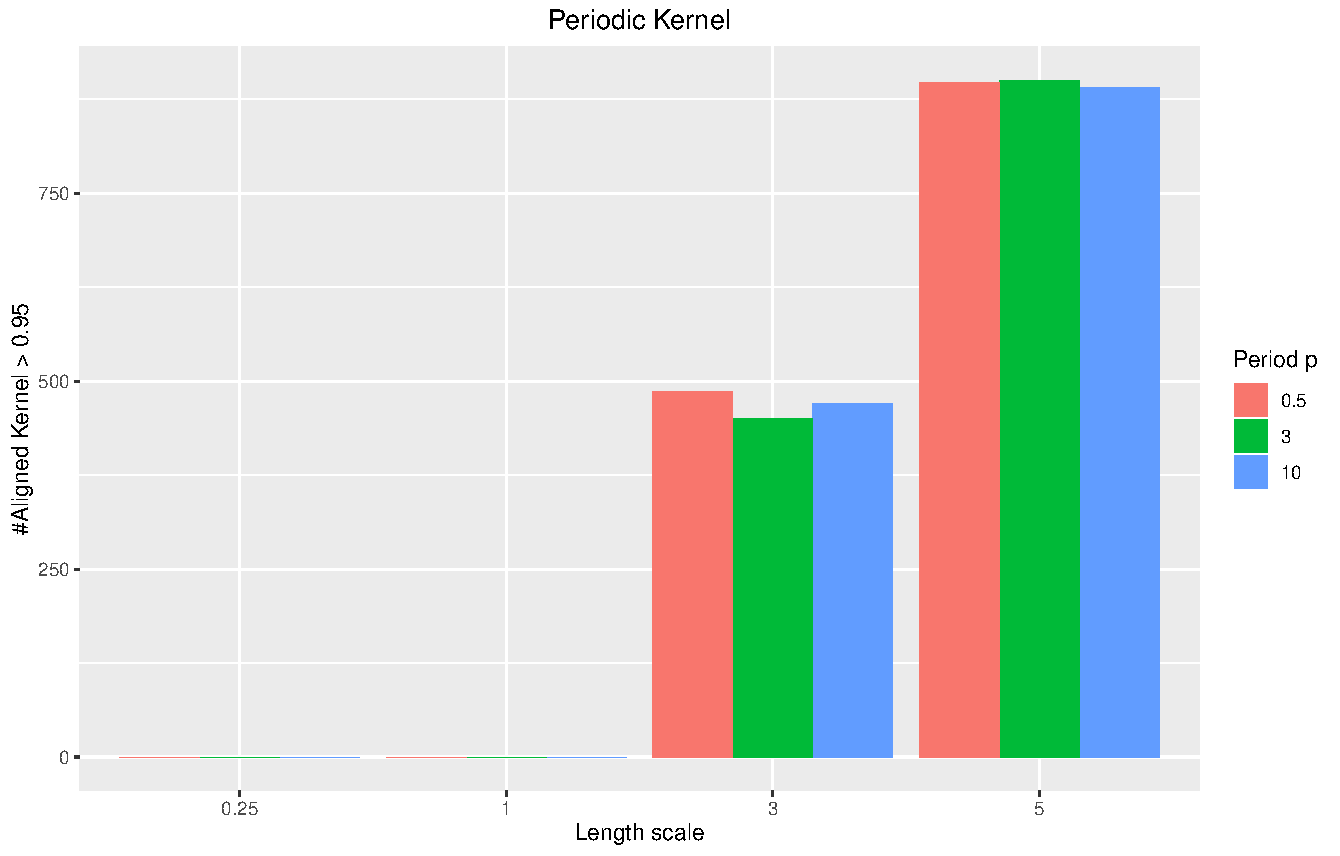
\includegraphics[width=0.8\textwidth]{Ex1_KPR.pdf}
            \caption[Periodic Kernel]%
            {{\small Periodic kernel}} 
        \end{subfigure}
        \quad
        \begin{subfigure}[b]{0.475\hsize}\centering
            \centering 
            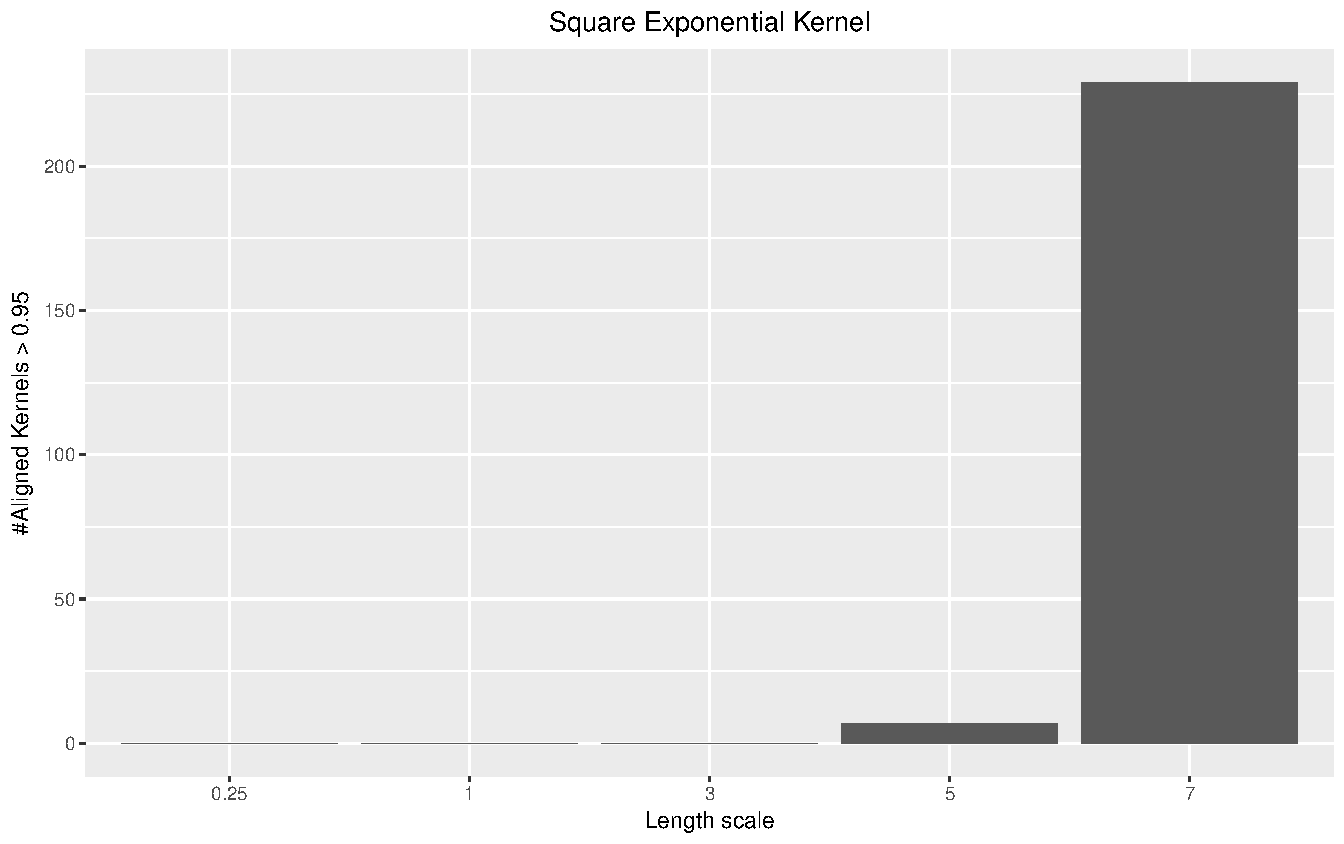
\includegraphics[width=0.8\textwidth]{Ex1_KSE.pdf}
            \caption[]%
            {{\small Square Exponential Kernel}}    
        \end{subfigure}
        \\
        \begin{subfigure}[b]{0.475\hsize}\centering   
            \centering 
            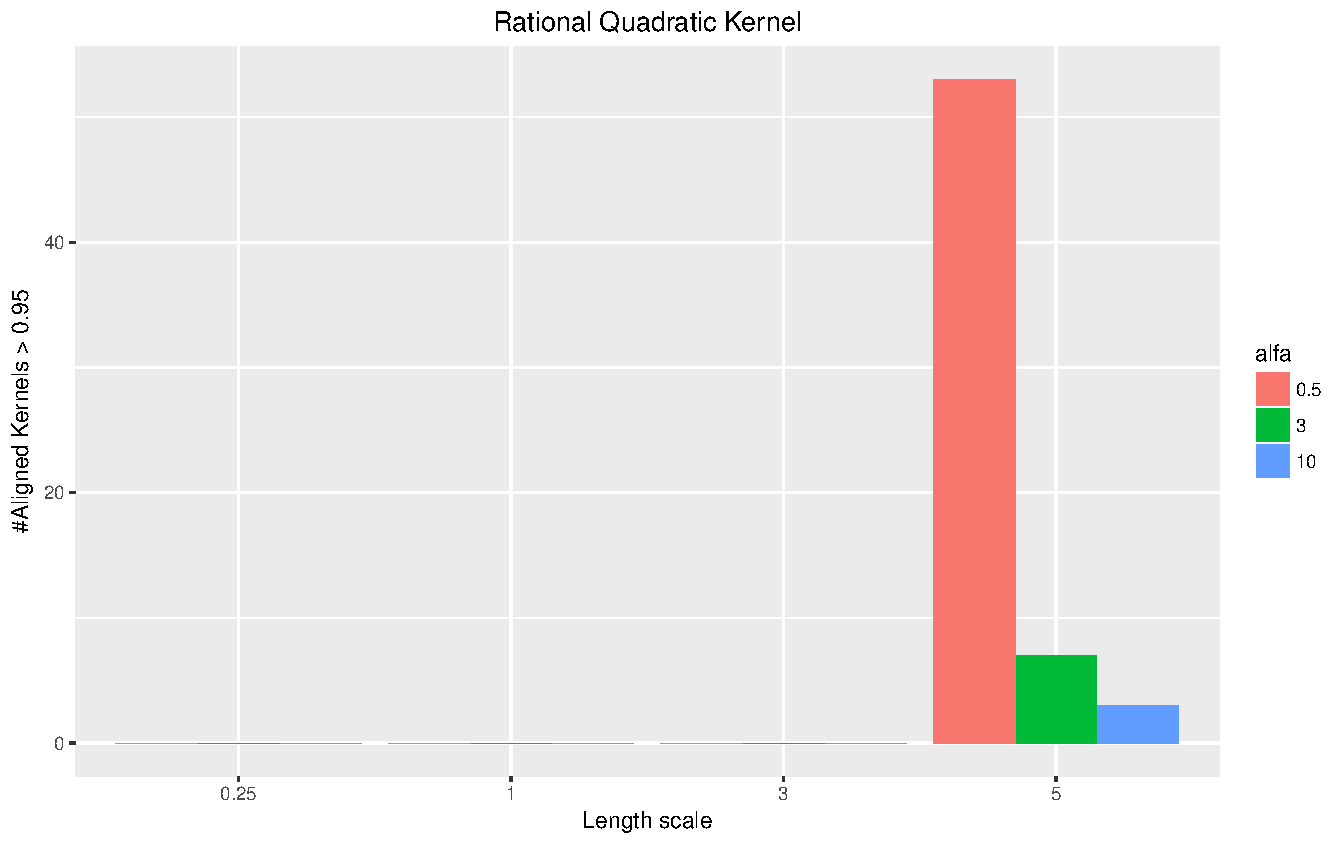
\includegraphics[width=0.8\textwidth]{Ex1_KRQ.pdf}
            \caption[]%
            {{\small Rational Quadratic Kernel}}
        \end{subfigure}
        \quad
        \begin{subfigure}[b]{0.475\hsize}\centering   
            \centering 
            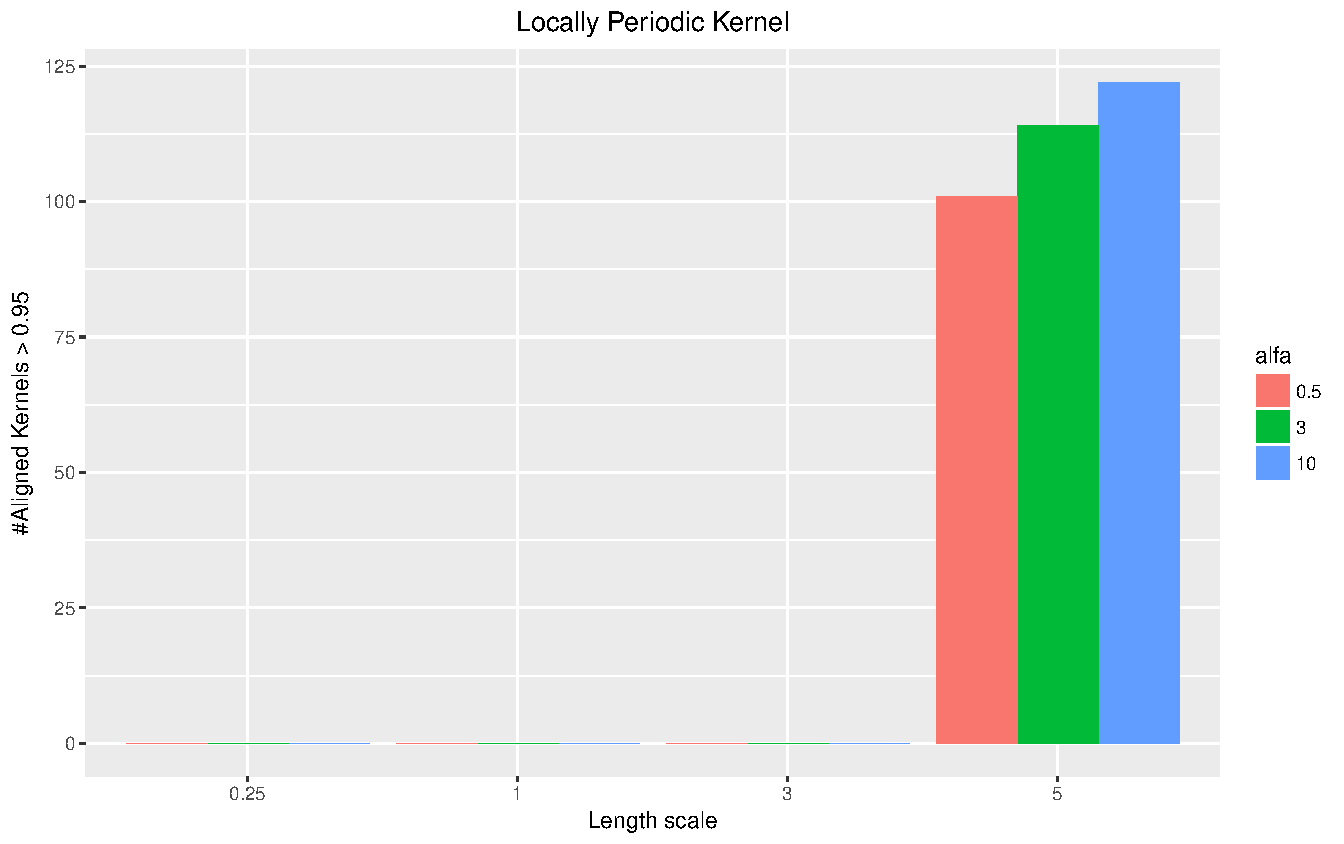
\includegraphics[width=0.8\textwidth]{Ex1_KlocPR.pdf}
            \caption[]%
            {{\small Locally periodic Kernel}}
        \end{subfigure}
        \caption[ Number of Kernel Aligned for each kernel family selected at level KTA $>$ 0.95. In the case of more than one hyperparameter considered, barplot are grouped according to the hyperparameter of interest ]
        {\small Number of Aligned Kernel for each kernel family selected at level KTA $>$ 0.95. In the case of more than one hyperparameter considered, barplots are grouped according to the hyperparameter of interest} 
        \end{figure*}
\end{landscape}

\restoregeometry 

\end{document}